\section{Introduction}

The concept of animal language hinges on the intricate ways through which non-human species communicate, revealing a spectrum of vocalizations, gestures, and behavioral cues that parallel human efforts to convey information and emotions. The study of animal communication has captivated researchers across numerous disciplines,
from biology to linguistics~\citep{rutz2023using,paladini2020bark,robbins2000vocal}. 
% \MY{refs needed here}
While it is widely accepted that most animals lack a language system comparable to human language,
recent advancements in natural language processing have opened up new avenues for investigating the patterns and structures embedded within animal vocalizations~\citep{huang2023transcribing,wang2023towards}. The study of animal language, therefore, not only broadens our understanding of the animal kingdom but also deepens our insights into the evolution and functions of communication systems across species.
% \MY{and here}
 
 
% \MY{This para needs to be combined with the next, and stress that there are already attempts to undercover acoustic variations of dog sounds, as illustrated in fig 1, at least 6 different types are found. Yet the definition of a language is more than different sound types, we are trying to find the minimal unit, which is phoneme, in dog sounds and then form into different ngrams}
%Dogs, species that have integrated into human society,offer a wealth of videos capturing their vocalizations and behaviors,which are readily available for scholarly investigation in today's video-centric online era. %Furthermore, numerous studies have already been 
%conducted in this domain.
% TODO

Despite observable acoustic variations in animal vocalizations that hint at potential patterns of communication, asserting that animals, such as dogs, possess a language is fraught with limitations. The absence of identifiable phonemes and structured syntax in their vocalizations challenges traditional linguistic frameworks~\citep{holdcroft1991saussure}. While dogs exhibit a range of sounds that vary in pitch, duration, and intensity, as illustrated in Figure \ref{fig:six_word} (sound clips extracted from Audioset~\citep{gemmeke2017audio}), six distinct dog barking sounds are identified. However,  these variations alone do not constitute a language. The lack of a structured, consistent phonetic system and the inability to form complex ideas through their sounds significantly limit the comparison of their vocalizations to human language.

%Prior research has predominantly concentrated on classification tasks rather than animal language comprehension,
%and studies pertaining to animal language transcription are confronted with two primary challenges.
%Furthermore, dog vocalizations sourced from online dog videos are typically accompanied by background music, noise, and sounds generated by the dog's interaction with its surroundings,
%thereby increasing the complexity of extracting dog vocalizations and analyzing dog vocalization patterns.

%---xy start

% 动机
%Verbal signs within a language have a shared denotation for members of the same linguistic group, acquired (together with many cultural connotations) through socialization~\citep{holdcroft1991saussure}.
%Language has a consistent pattern and is a symbol of certain meanings. We are curious if dogs have a language and what communication patterns they use. 
% \KZ{We can show a figure here to the audio wave and spectrograms of the 6 diff
% dog word types, to indicate that the six kinds of dog barks have distinct
% acoustic features. This gives rise to our idea of using HuBert to find the 
% distributional representation of the dog sounds (phones).}
%Past work~\citep{gemmeke2017audio} has indicated that there are six distinct categories of dog sounds. They have distinct acoustic features(\figref{fig:six_word}). This is subjective, there may be more varieties of dog language.

\begin{figure}[th]
    \centering
    \scalebox{0.35}{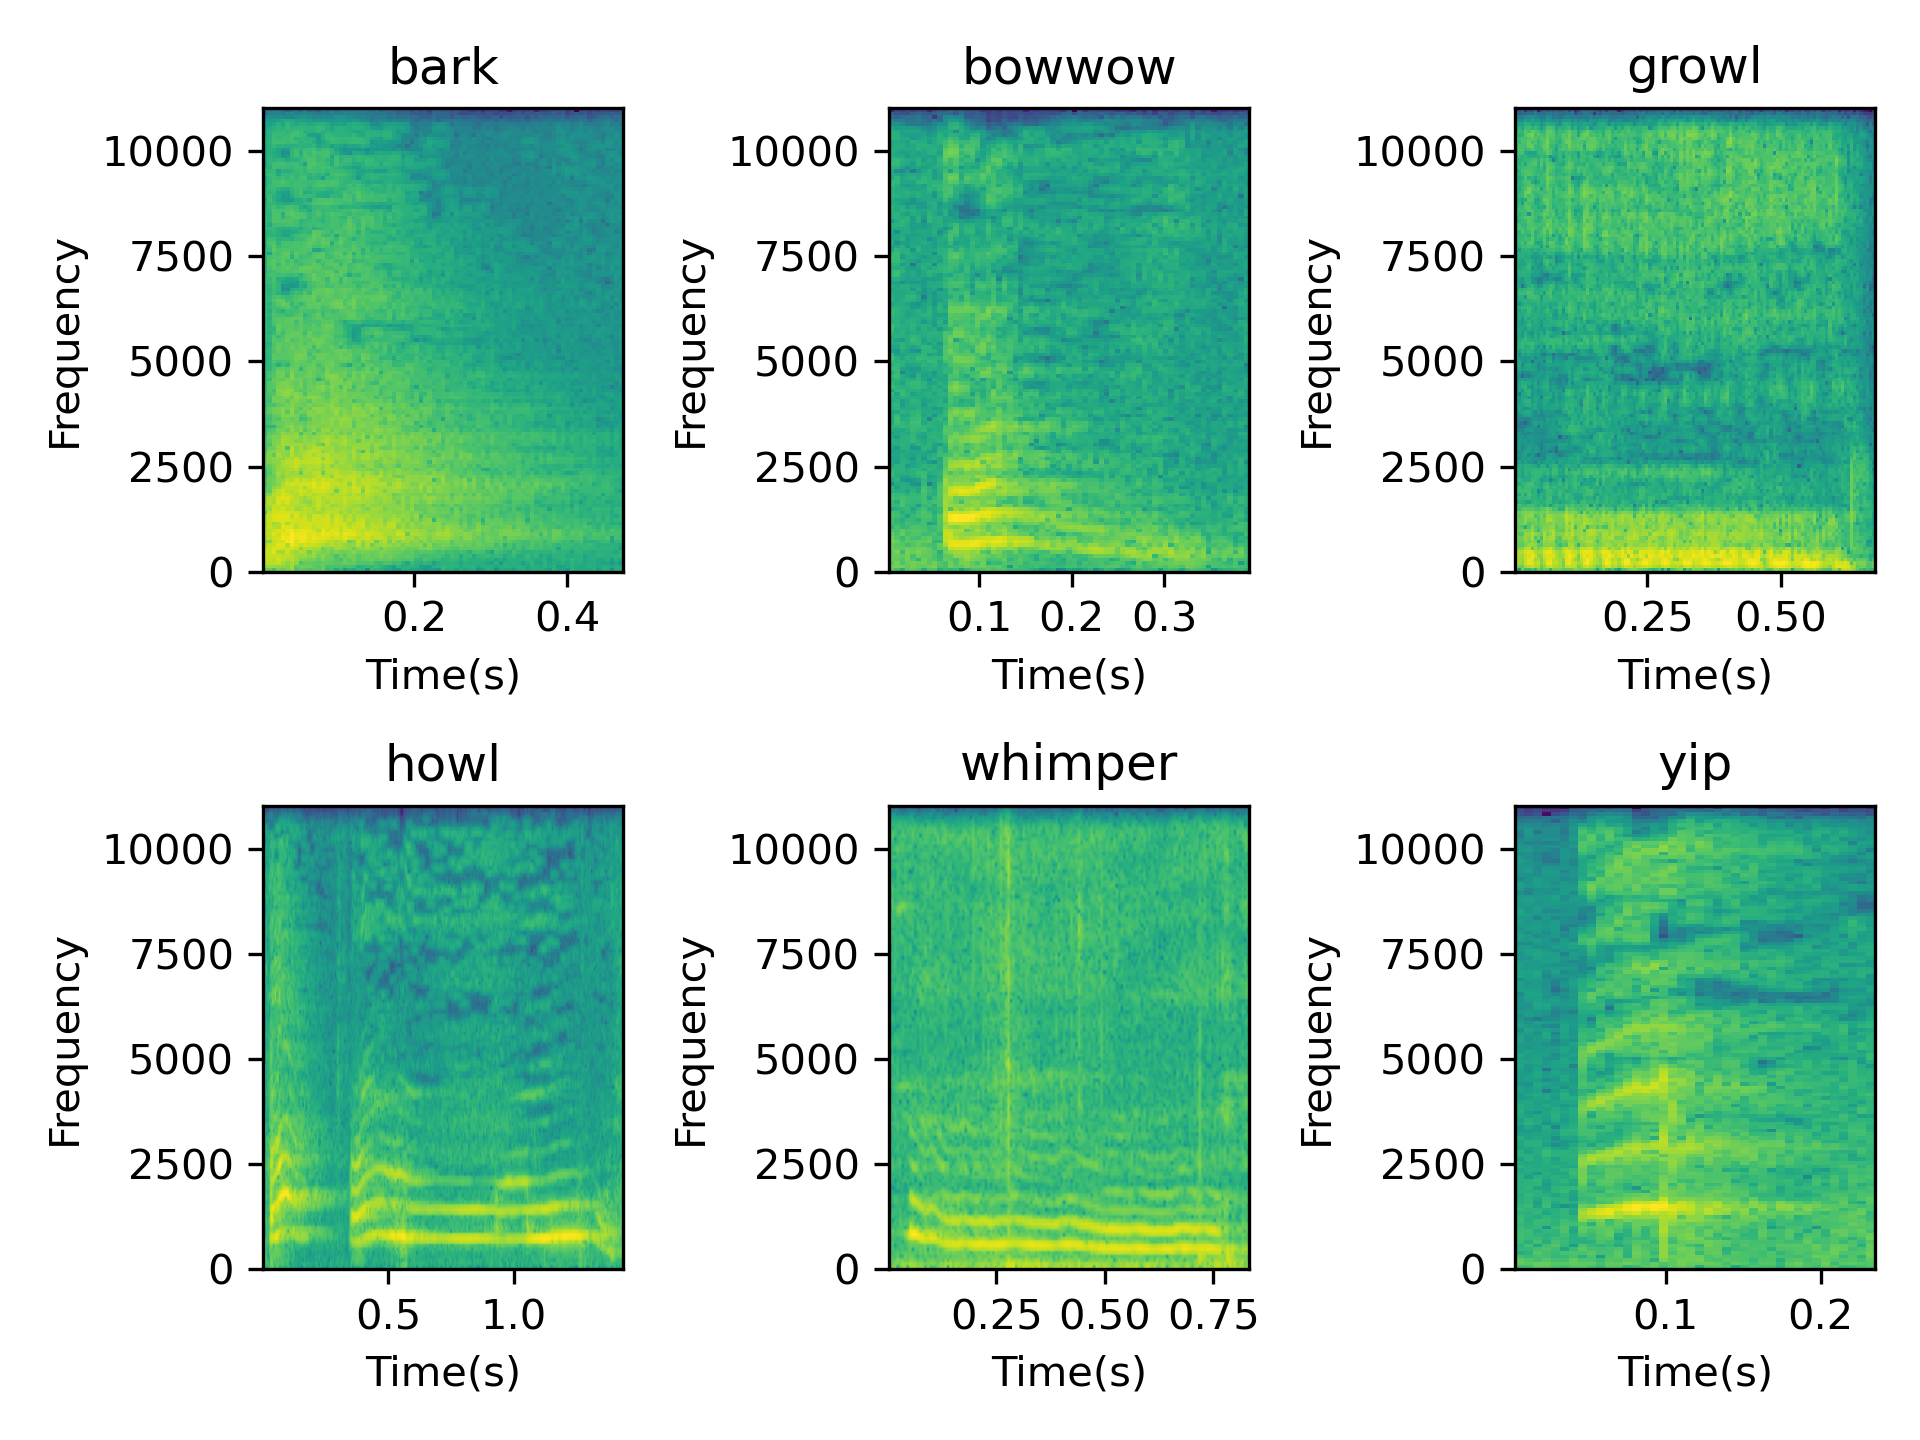
\includegraphics{six_word.png}}
    \caption{Six different dog barking sounds from AudioSet~\citep{gemmeke2017audio}}
    \label{fig:six_word}
\end{figure}

%To uncover the vocabulary in ``dog language'' capable of effectively conveying information,
%a fundamental requirement is that the vocalization of the word can be produced by multiple dogs and must possess statistical significance before it can be classified as a word within ``dog language''.\MY{your point is there, but scattered here and there, logically combine these small paragraphs and make it into one. think about what you wanna say}

% 挑战
Nevertheless, undertaking the challenge of exploring the concept of animal language is a daunting task. Different from well-researched human language, the frequency range, and phonetic variations remain under-discovered, rendering the classification approach based on sound amplitude inadequate for discerning the fundamental phonemes of dog vocalizations. The difficulty lies not only in interpreting the acoustic variations but also in identifying meaningful patterns within the vast array of animal sounds. This complexity is compounded by the need to distinguish between mere noise and significant vocalizations that could indicate some form of structured communication. The endeavor requires innovative methodologies and a departure from traditional linguistic analysis. 
%Discovering the vocabulary of ``dog language'' that fulfills the above requirements is a huge challenge. 
%1) \textbf{Unknown acoustic traits}. %due to dog vocalizations exhibiting phonetic variations on segment and supra-segmental levels, we assume that we can assign phoneme labels to different sounds.

%the combination of distinct phonemes inevitably alters the pronunciation of each phoneme to some extent, thereby posing a challenge for audio-based classification methods to group identical phonemes into a single category; 2) \MY{can you summarize a small bullet point for the second challenge? this is not clear by far. are you saying that we are difficult to ascertain the definition of a word?} it is not feasible to ascertain the vocabulary present within ``dog language'' solely based on acoustic features. 
%We also need to categorize identical words uttered by different dogs, despite subtle variations (among individual dogs), into a single group. Concurrently, it is imperative to ensure that the ``word'' constitutes an uninterrupted vocalization, produced in a single breath.

% % 注释v1 start
% First, the identification and summarization of fundamental units in dog vocalizations pose a significant difficulty. 
% \MY{units need better definitions here, i.e. fundamental frequencies, duration, sound patterns}
% % \MY{Different from well-researched human language, the frenquency range, phonetic variations remain under discovered}
% % Given the absence of prior knowledge, both the types and durations of these basic units remain undetermined,
% Different from well-researched human language, the frequency range, and phonetic variations remain under-discovered, rendering the classification approach based on sound amplitude inadequate for discerning the fundamental phonemes of dog vocalizations. 
% % Moreover, as sound itself is continuous,
% % the combination of distinct phonemes inevitably alters the pronunciation of each phoneme to some extent, \MY{we are making an assumption here, that dog vocalizations exhibit phonetic variations on segment and supra-segmental levels, hereby we can assign phoneme labels to different sounds. }
% % thereby posing a challenge for audio-based classification methods to group identical phonemes into a single category.
% % 改成下面这个
% Due to dog vocalizations exhibiting phonetic variations on segment and supra-segmental levels, we assume that we can assign phoneme labels to different sounds. As sound itself is continuous,
% the combination of distinct phonemes inevitably alters the pronunciation of each phoneme to some extent, thereby posing a challenge for audio-based classification methods to group identical phonemes into a single category.

% Second, it is not feasible to ascertain the vocabulary present within ``dog language'' solely based on acoustic features. To uncover the vocabulary in ``dog language'' capable of effectively conveying information,
% a fundamental requirement is that the vocalization of the word can be produced by multiple dogs 
% % \MY{consistent patterns, find the definition of language with refs, that sounds are symbols to signify certain meanings.} 
% and must possess statistical significance before it can be classified as a word within ``dog language''. It has a consistent pattern and is a symbol of certain meanings.
% This necessitates our ability to categorize identical words uttered by different dogs, despite subtle variations (among individual dogs), into a single group. Concurrently, it is imperative to ensure that the ``word'' constitutes an uninterrupted vocalization, produced in a single breath.
% % 注释v1 end

% 说明为我们为解决挑战所作的工作
Our approach to navigating these challenges involves leveraging advanced signal processing techniques and self-supervised learning models. By focusing on the acoustic features of dog vocalizations, we aim to uncover underlying patterns that could suggest a rudimentary form of communication. This involves a meticulous process of audio clean-up, sentence extraction, phoneme recognition and combination, and the establishment of word discovery across vocalizations from different individual dogs. Given the lack of prior knowledge of dog vocalizations, we apply a self-supervised approach HuBERT~\citep{hsu2021hubert} for pretraining and phoneme identification.
HuBERT can effectively reference the context information of the audio and generate vector representations, which enables it to generate stable results when faced with vocalizations like language that may have slight variations in context. 

Utilizing the precise phoneme labels acquired, we explored the feasibility of creating a vocabulary from the available dog sound dataset, characterized by complete and commonly occurring phoneme sequences vocalized by numerous dogs, which could be identified as a ``word''.
We developed popularity score to quantify the likelihood of a phoneme ngram constituting a ``word'', assessing the vocabulary's validity through its precision in human evaluation of vocalization completeness and its recall by determining the coverage rate within dog vocalization sequences. Our analysis revealed acoustic uniformity in the segments of identical phoneme ngrams across various dogs, demonstrating that these ``words'' comprehensively encompass the entirety of dog vocalization sentences.


%To address the first challenge, we apply a self-supervised approach rather than a priori knowledge of human language, building on the work of \citet{huang2023transcribing}.\MY{can you combine these 3 paragraphs?}

%To address the first challenge, Our work follows and optimizes the process of dog data processing by \citet{huang2023transcribing}. We apply a self-supervised approach~\citep{hsu2021hubert} rather than a priori knowledge of human language. Given the lack of prior knowledge of dog vocalizations, a self-supervised approach is more appropriate.
%HuBERT can effectively reference the context information of the audio and generate vector representations, which enables it to generate stable results when faced with vocalizations like language that may have slight variations in context.

%Based on the accurate phoneme labels obtained, we considered whether it is possible to establish a vocabulary from the existing dog sound dataset, which contains complete and frequent phoneme sequence combinations uttered by multiple individuals, and we can call it a ``word''. To address the second challenge, We designed a popularity score to measure the probability of a phoneme ngram being considered a ``word'', and we measured the reliability of the ``vocabulary'' by its precision on human testing whether it is a complete vocalization and recall by calculating ``vocabulary'' coverage rate on dog vocalization sentences. We find that the vocalization segments of the same phoneme ngram have acoustic consistency in the vocalizations emitted by multiple dogs, and that these ``words'' can cover 100\% of the dog sound sentence.

% % 注释v2 start
% Our work follows and optimizes the process of dog data processing by \citet{huang2023transcribing}
% % \MY{why citeposs? usually citep or citet, read their differences before use}. 
% We intercepted segments containing dog voices using PANNs~\citep{kong2020panns} and extracted dog vocalization segments from audio with complex sound sources using AudioSep~\citep{liu2023separate}. We segmented the dog vocalization sentences according to the silent segments in audio clips. Since transformer-based models can extract audio context information very well, we pre-trained the HuBERT~\citep{hsu2021hubert} model with processed dog vocalization sentences and tested its results on the downstream task of dog vocalization type classification using the test dataset, and obtained the optimal number of classifications. The HuBERT model can effectively reference the context information of the audio and generate vector representations, which enables it to generate stable results when faced with vocalizations like language that may have slight variations in context. 

% % We clustered the approximately 20ms basic phonemes generated by HuBERT and obtained the labels for each phoneme, which showed good consistency under human cognitive testing. In other words, the acoustic features of phonemes with the same label are similar, while the acoustic features of phonemes with different labels are significantly different. \MY{This is too detailed for introduction, what we should stress is that without ample knowledge to label dog vocalizations, self-supervised learning is an appropirate choice and say that compared to hubert on humans, what we do is xxxx}
% % 改成下面的
% Some works~\citep{huang2023transcribing,wang2023towards} in the past used a priori knowledge of human languages that may not apply to dog vocalizations. Given the lack of prior knowledge of dog vocalizations, a self-supervised approach is more appropriate.
% Based on the accurate phoneme labels obtained, we considered whether it is possible to establish a vocabulary from the existing dog sound dataset, which contains complete and frequent phoneme sequence combinations uttered by multiple individuals, and we can call it a ``word''. We designed a popularity score to measure the probability of a phoneme ngram being considered a ``word'', and we measured the reliability of the ``vocabulary'' by its precision on human testing whether it is a complete vocalization and recall by calculating ``vocabulary'' coverage rate on dog vocalization sentences. We find that the vocalization segments of the same phoneme ngram have acoustic consistency in the vocalizations emitted by multiple dogs, and that these ``words'' can cover 100\% of the dog sound sentence.
% During the experiment, we developed a web-based dog sound labeling system that can process dog vocalization clips uploaded by users, label them based on vocalization features, and display them. Users can observe and listen to dog vocalization clips with the same label and the segmentation of ngrams appearing in the ``vocabulary''. The system also provides some pre-trained sound clips and corresponding video clips, which is convenient for us to further discover the meaning of dog ``vocabulary'' through video. \MY{Intro is lengthy, make sure each paragraph serves one point, and every paragraph is connected logically between each other. Motivation, challenge, contribution.}
% % 注释v2 end

Our contributions lie in three aspects: 
\begin{enumerate}
\item We developed a robust processing pipeline for dog vocalizations, achieving high accuracy in phoneme labeling.
%we introduce a reliable
% \MY{this is a difficult to evidence adjective, give stats if you have, to show that your method is more reliable than previous ones} 
%dog language processing pipeline and obtain accurate dog vocalization phoneme labels; 
\item We design a popularity score to measure the probability of a dog phoneme ngram being a dog word, and obtain a vocabulary of dog phonemes without repetition. These words are uttered by multiple dogs and exhibit significant consistency.
\item We developed a web-based dog vocalization labeling system that can analyze and label dog audio uploaded by users, and highlight phoneme ngrams present in the vocabulary, laying an important foundation for further research on dog language understanding.
\end{enumerate}
